\documentclass[11pt,a4paper,headings=standardclasses]{scrartcl}
%%%%%%%%%%%%%%%%%%
%%Switch on and of solutions with (un-)commenting
%%the following line
%%%%%%%%%%%%%%%%%%
%\def\modelsolution{1}

\newcommand{\solution}[1]{
  \ifx\modelsolution\undefined
  \else
    \par{\bfseries\em Lösung: } #1
  \fi
}

\usepackage{scrlayer-scrpage}
\usepackage{anysize}
%\usepackage[final]{graphicx}
\usepackage{float} 
\setlength{\parindent}{0em}
\setlength{\parskip}{1ex plus 1pt}


\usepackage[compat=1.1.0]{tikz-feynman}
\usetikzlibrary{calc}
\newcommand{\XA}{3}
\newcommand{\YA}{1}

\usepackage{booktabs}
  \usepackage[
    locale=DE,
    separate-uncertainty=true,
    per-mode=symbol-or-fraction,
  ]{siunitx}

\DeclareSIUnit\barn{b}

\ofoot[\pagemark]{\pagemark}
\cfoot[\bfseries Klausur zur KET-Vorlesung im WS~2022/23, TU Dortmund]{\bfseries Klausur zur KET-Vorlesung im WS~2022/23, TU Dortmund}
\lohead[{Name: \rule[0em]{15em}{1pt}}]{Name: \rule[0em]{15em}{1pt}}
\rohead[{Matrikelnr: \rule[0em]{8em}{1pt}}]{Matrikelnr: \rule[0em]{8em}{1pt}}

\setkomafont{pageheadfoot}{%
  \normalfont\normalcolor
}
\setkomafont{pagenumber}{\normalfont\bfseries}


  
\usepackage[ngerman]{babel}

\usepackage{amsmath}
\usepackage{mathtools}
\usepackage{amssymb}
\usepackage{braket}
\usepackage{icomma}
\usepackage{csquotes}
\usepackage{cancel}
\usepackage{enumerate}
\usepackage{enumitem}

%\usepackage{epsfig}
\usepackage[final]{pdfpages}
\usepackage{ifthen}

\usepackage{helvet}
\usepackage{palatino}
\usepackage{mathpazo}
\usepackage{feynmf}\unitlength=1mm
\usepackage{isotope}
\usepackage{polyglossia}
\usepackage[version=4]{mhchem}
\setmainlanguage{german}

\usepackage{fontspec}
\defaultfontfeatures{Ligatures=TeX}
\usepackage{placeins}
\usepackage{version}

\pagestyle{scrheadings}

\clubpenalty = 10000
\widowpenalty = 10000


\renewcommand{\labelenumi}{(\alph{enumi})}
\renewcommand{\theenumi}{(\alph{enumi})}%
\renewcommand{\labelenumii}{\arabic{enumii}.}

\newcommand{\del}{\partial}
\newcommand{\rot}{\mathop{\rm rot}\nolimits}
\newcommand{\grad}{\mathop{\rm grad}\nolimits}
\renewcommand{\Re}{\mathop{\rm Re}\nolimits}
\renewcommand{\Im}{\mathop{\rm Im}\nolimits}


%Aufgabenumgebung
\newcounter{punkte}
\newcounter{aufgabenr}
\setcounter{aufgabenr}{1}

\newcounter{loopcounter}
\newcommand{\forloop}[5][1]% 
{% 
  \setcounter{#2}{#3}% 
  \ifthenelse{#4}% 
  {% 
    #5% 
    \addtocounter{#2}{#1}% 
    \forloop[#1]{#2}{\value{#2}}{#4}{#5}% 
  }% 
  % Else 
  {% 
  }% 
}% 

\newcounter{endcounter}
\newboolean{Musterlsg}


\newenvironment{aufgabe}[3]{ %\aufgabe{#freieSeiten}{Titel}{Punkte}
  {\cleardoubleoddplainpage 
   \vspace*{1em}
   \Large{\bfseries \sffamily Aufgabe \arabic{aufgabenr}: #2
  \hfill (#3 Punkte)}} \par
  \setcounter{endcounter}{#1}
}{
  \stepcounter{aufgabenr}
  \ifthenelse{\boolean{Musterlsg}}{
  }
  { 
    %Keine Musterlsg
    \forloop{loopcounter}{0}{\value{loopcounter} < \value{endcounter}}{\clearpage\mbox{}}
  }
}

\newenvironment{loesung}{
   \vspace{2em} {\large \sffamily \bfseries L\"osung:} \nopagebreak[4]
}{}

\begin{document}
  \begin{titlepage}
    \titlehead{\Large TU Dortmund \hfill WS~2022/23}
    \subject{Klausur}
    \title{Einführung in die Kern- und Elementarteilchenphysik}
    \author{Prof.~Dr.~Johannes Albrecht}
    \date{15. Februar 2023}
    \maketitle
    {
      \thispagestyle{empty}
      \centering
      \large
      \begin{tabular}{lp{0.7\linewidth}}
        Name:           & \dotfill \\[1em]
        Matrikelnummer: & \dotfill \\[1em]
        Übungsgruppe:   & \dotfill \\[1em]
        Studiengang:    & \dotfill \\[1em]
      \end{tabular}
      \textbf{Schreiben Sie Ihren Namen und Ihre Matrikelnummer auf jedes Blatt!} \\[8mm]
      {
        \large
        \begin{tabular}{|l|c|c|c|c|c|c|c|c|c|c|c|}
          \hline
          Aufgabe & 1 & 2 & 3 & 4 & 5 & 6 & 7 & $\Sigma$& Ausweiskontr.
          \parbox[0pt][2em][c]{0cm}{} \\
          \hline
          Punkte & \hspace*{0.05\linewidth}
                 & \hspace*{0.05\linewidth}
                 & \hspace*{0.05\linewidth}
                 & \hspace*{0.05\linewidth}
                 & \hspace*{0.05\linewidth}
                 & \hspace*{0.05\linewidth}
                 & \hspace*{0.05\linewidth}
                 & \hspace*{0.05\linewidth}
                 & \parbox[0pt][2em][c]{0cm}{} \\
          \hline
        \end{tabular}
      } \\[1em]
      \begin{tabular}{ll}
        Voraussetzung: & erfolgreiche Teilnahme an den Übungen \\
        Punktzahl:     & max. 80 Punkte, 70 Punkte entsprechen 100\%, \\
                       & die Klausur gilt ab 28 erreichten Punkten als sicher bestanden. \\
        Dauer:         & 3 Stunden
      \end{tabular}
    }
    \vfill
    \textbf{\sffamily Zugelassene Hilfsmittel:}
    \begin{itemize}
      \item gewöhnlicher, nicht grafikfähiger Taschenrechner
      \item ein einseitig beschriebenes DIN-A4-Blatt mit handgeschriebenen Formeln
    \end{itemize}
    \begin{center}
      \textbf{Viel Erfolg!}
    \end{center}
    \vfill
    \begin{center}
      \fbox{\parbox[c]{0.95\textwidth}{
        \textbf{Bitte lesen und unterschreiben Sie die Erklärung auf Seite 2  des Titelblattes.}
      }}
    \end{center}
    \newpage
    \begin{center}
      \fbox{\parbox[c]{1\textwidth}{
        \textbf{Die folgende Erklärung bitte \emph{vor Klausurbeginn} lesen und unterschreiben:} \\[0.5em]
        Ich habe zur Kenntnis genommen, dass die Fakultät Physik diese Klausur nur bis zum 15.5.2023 aufbewahrt,
        falls ich sie nicht nach der Klausureinsicht persönlich in Empfang nehme.
        Nach diesem Zeitpunkt wird nur dieses Deckblatt mit persönlichen Angaben,
        Klausurergebnis und Note archiviert, die Aufgabenblätter werden vernichtet. \\[2ex]
        Ich habe zur Kenntnis genommen, dass eine nicht bestandene
        Modulprüfung in einem Pflichtmodul des Studiengangs Medizinphysik/Physik
        spätestens nach 13 Monaten wiederholt werden muss. \\[2ex]
        $\Box$ Ich bin \textbf{NICHT} damit einverstanden, dass meine Note unter
        Angabe meiner Matrikelnummer online im moodle veröffentlicht wird (falls zutreffend: ankreuzen). \\[5ex]
        (Unterschrift)\ \hrulefill
      }}
      
      
      \fbox{\parbox[c]{1\textwidth}{
      \textbf{Identitätsprüfung:} Ich versichere an Eides statt, dass ich durch ordnungsgemäße Anmeldung berechtigt bin, die nachfolgende Prüfung zu absolvieren, und dass ich sie selbst ablegen werde. Mir ist bewusst, dass eine Verletzung dieser eidesstattlichen Versicherung strafrechtliche Konsequenzen hat. \\
      
    \textbf{Eigenständigkeitserklärung: }Ich versichere an Eides statt, dass ich die nachfolgende Prüfung selbstständig und ohne Hilfe Dritter absolvieren sowie keine anderen als die genannten und explizit zugelassenen Hilfsmittel verwenden und mich im Allgemeinen prüfungskonform verhalten werde. Mir ist bewusst, dass Täuschungsversuche nach der für mich geltenden Prüfungsordnung geahndet werden.\\
    
    \textbf{Prüfungsfähigkeit: }Ich versichere an Eides statt, dass ich prüfungsfähig bin.
\\[5ex]
        (Unterschrift)\ \hrulefill
      }}

\vfill
      
      \fbox{\parbox[c]{1\textwidth}{
        \textbf{Die folgende Erklärung bitte \emph{bei Klausurrückgabe} lesen und unterschreiben:} \\[0.5em]
        Hiermit bestätige ich den Erhalt meiner vollständigen Klausur. Ich erkenne das Ergebnis und die Note an. \\[2ex]
        (Unterschrift)\ \hrulefill
      }}
    \end{center}
  \end{titlepage}

%\thispagestyle{empty}
\section*{Formeln, Konstanten}
Neben den hier aufgef\"uhrten Gr\"o{\ss}en finden Sie am Ende der Klausur eine Clebsch-Gordan-Tabelle und eine Liste von Teilchen und ihren Eigenschaften.

\begin{align*}
 c &= \SI{3e8}{m/s} \\
 \hbar &= \SI{1.055e-34}{Js} \\ &= \SI{6.582e-22}{MeV s}\\
 e &= \SI{1.6022e-19}{C} \\ 
 \frac{G_F}{(\hbar c)^3} &= \SI{1.166e-5}{GeV^{-2}} \\
 \alpha &= 1/137 \\
 N_A &= \SI{6.022e23}{mol^{-1}} \\
 \theta_C &= 0.22 \, {\text{ rad}} \\
 \epsilon_0 &= \SI{8.8541e-22}{\farad \metre^{-1}} \\ &= \SI{55.263}{e^2 eV^{-1} \micro m^{-1}} \\
\end{align*}
Die Einträge der CKM-Matrix lauten:
\begin{align*}
    V_\text{CKM} &= 
      \begin{pmatrix}
      V_{ud} & V_{us} & V_{ub} \\
      V_{cd} & V_{cs} & V_{cb} \\
      V_{td} & V_{ts} & V_{tb}
  \end{pmatrix}
\end{align*}
mit
\begin{align*}
 (|V_{ij}|) \approx
  \begin{pmatrix}
      1         & 0,2   & 0,008 \\
      0,2     & 1       & 0,04 \\
      0,008 & 0,04 & 1
  \end{pmatrix}
\end{align*}
Die Bethe-Weizs\"acker-Formel lautet:
\begin{align*}
E_\text{Bindung}\approx15,67\,\text{MeV}\cdot A - 17,23\,\text{MeV}\cdot A^{\frac 2 3} - 0,71\,\text{MeV}\cdot Z\cdot(Z-1) \cdot A^{-\frac 1 3} -  93,15\,\text{MeV}\cdot \frac{(N-Z)^2}{4A} + E_\text{Paar}
\end{align*}
mit
\begin{align*}
E_\text{Paar} = 
   \begin{cases}
     +11,2\,\text{MeV}\cdot A^{-\frac 1 2} & \text{f\"ur gg-Kerne}\\
     0  & \text{f\"ur ug- und gu-Kerne}\\
     -11,2\,\text{MeV} \cdot A^{-\frac 1 2} & \text{f\"ur uu-Kerne} 
   \end{cases}
\end{align*}

Einige Land\'e-Faktoren:\\
\centerline{\begin{tabular}{lc}\hline
Teilchen & $g$ \\ \hline
Elektron & -2.0023 \\
Myon     & -2.0023 \\
Neutron  & -3.8261 \\
Proton   & +5.5857 \\ \hline
\end{tabular}}

Abgestrahlte Leistung eines Teilchens: 
\begin{equation}
    P = \frac{e^2c}{6\pi\epsilon_0(m_0c^2)^4}\frac{E^4}{R^2}
\end{equation}

\cleardoubleemptypage
\setcounter{page}{1}
\pagestyle{scrheadings}

\section{Kurzfragen - (20P)}
\begin{enumerate}
\item Was sind die magischen Zahlen und wie verhält sich die Bindungsenergie in der Nähe der magischen Zahlen? (2P)

\vspace{3cm}\item Nennen Sie zwei Kenngrößen eines Beschleunigers. (2P)

\vspace{3cm}\item Welche Strahlungsart wird bei einem Übergang von $\ce{^{224}Ra} \rightarrow \ce{^{220}Rn}$ frei? Welcher Kernprozess liegt diesem Übergang zugrunde? (2P)

\vspace{3cm}\item Wodurch ist die maximale Energie, auf die ein Teilchen beschleunigt werden kann, bei einem Linearbeschleuniger limitiert? (2P)

\vspace{4cm}\item Welche zwei Eigenschaften muss ein Kandidat für ein Dunkle-Materie-Teilchen haben? (2P)

\vspace{3cm}\item Sind Flavour-Changing-Neutral-Currents (FCNC) im Standardmodell auf Tree-Niveau erlaubt? Begründen Sie Ihre Antwort. (2P)

\vspace{3cm}\item Vergleichen Sie die CKM- mit der PMNS-Matrix. Nennen Sie mindestens eine Gemeinsamkeit und einen Unterschied. (2P)

\vspace{3cm}\item Was ist eine additive Quantenzahl? Nennen Sie zwei Beispiele. (2P)


\vspace{3cm}\item Welche der folgenden Reaktionen sind im Standardmodell verboten, welche sind erlaubt?
Begründen Sie Ihre Entscheidungen. Geben Sie mögliche Wechselwirkungen
für die erlaubten Prozesse an. Nehmen Sie an, dass Neutrinos masselos sind.  
Zeichnen Sie die dominanten Feynman-Diagramme für die erlaubten Prozesse.
Geben Sie dabei alle intermediären Teilchen an. (4P)

\begin{itemize}
    \item $\mu^- \to e^- \gamma $
    \item $B_s \to \mu^+ \mu^- \gamma $
    \item $B_s \to \phi \phi$
    \item $n \to p  e^- \bar{\nu_e}$
\end{itemize}

\end{enumerate}

\null\newpage\clearpage
\newpage
\null\newpage

\section{Beschleuniger und Detektoren (10P)}

\begin{enumerate}
\item Beschreiben Sie \textit{kurz} die Vor- und Nachteile von Elektron- und Protonbeschleunigern. Welche Beschleunigerarten werden für gewöhnlich für die beiden Teilchenarten genutzt? Begründen Sie Ihre Antwort. (2P)
\solution{
\textit{2 Punkte.}
      \begin{itemize}
          \item Protonen
          \begin{itemize}
              \item Pro
              \begin{itemize}
                  \item Hohe Masse, wenig Synchrotronstrahlung
              \end{itemize}
              \item Contra
              \begin{itemize}
                  \item Zusammengesetztes Teilchen, einzelne Partonen haben geringere Energie
              \end{itemize}
              \item Beschleuniger
              \begin{itemize}
                  \item Im Prinzip alle, jedoch bieten sich Kreisbeschleuniger an, da Protonen wenig Energie über Synchrotronstrahlung verlieren
              \end{itemize}
          \end{itemize}
          \item Elektron
          \begin{itemize}
              \item Pro
              \begin{itemize}
                  \item Stabiles Elementarteilchen
              \end{itemize}
              \item Contra
              \begin{itemize}
                  \item Geringe Masse, viel Synchrotronstrahlung
              \end{itemize}
              \item Beschleuniger
              \begin{itemize}
                  \item An sich ist auch hier alles möglich, jedoch bieten sich für Colliderexperimente am ehesten Linearbeschleuniger an, da hier keine Energie durch Synchrotronstrahlung verloren wird.
              \end{itemize}
          \end{itemize}
      \end{itemize}
  }

  \item Gegeben sei nun ein - natürlich nur rein hypothetischer - Kreisbeschleuniger mit einem Radius von $R = \SI{16}{\kilo \metre}$, der mit einer Strahlenergie von $E =\SI{50}{\tera \electronvolt}$ betrieben wird. Bei einem Durchlauf durch den Beschleuniger verlieren die beschleunigten Teilchen durch Synchrotronstrahlung $\SI{2.6(1.0)}{\tera \electronvolt}$ Energie. Berechnen Sie mit diesen Informationen die untere und obere Massengrenze des beschleunigten Teilchens. Um welches Teilchen handelt es sich? (3P) 
  \solution{
  \textit{3 Punkte.} \\
  Es gilt der Zusammenhang:
              \begin{equation}
                  P = \frac{e^2c}{6\pi\epsilon_0(m_0c^2)^4}\frac{E^4}{R^2}
              \end{equation}
              Daher ergibt sich die Energie für einen Umlauf durch:
              \begin{eqnarray}
                  E_{\text{syn}} = \int Pdt = Pt = P\frac{2\pi R}{c} &= \frac{e^2}{3\epsilon_0(m_oc^2)^4}\frac{E^4}{R} \\
                  &= C \cdot (\frac{(m_oc^2)}{E})^4 \cdot \frac{1}{R}
              \end{eqnarray}
              Die Konstante $C$ ergibt sich zu
              \begin{eqnarray}
                  C = \frac{e^2}{3\epsilon_0} &=& 9.66\cdot10^{-28}\,\frac{\mathrm{C^2Vm}}{\mathrm{As}}\\
                  &=& 6.031\cdot 10^{-9}\,\mathrm{eVm}
              \end{eqnarray}
              Damit ergibt sich für die Masse der folgende Zusammenhang:
              \begin{equation}
                  m = \left( \frac{C}{R \cdot E_{\text{syn}}} \right)^\frac{1}{4} E.
              \end{equation}
              Mit eingesetzten Werten erhält man ein Massenspektrum von ca. ${900-1100} \,\si{\mega \electronvolt}$. Es handelt sich daher um Protonen oder Neutronen. Neutronen können aufgrund ihrer Ladung jedoch ausgeschlossen werden.
  }
\end{enumerate}
Sie wollen nun einen Detektor für den potentiellen Zerfall $X\rightarrow \Sigma^0 \ell^+ \ell^-?$ bauen, wobei das $\Sigma^0$-Teilchen in $\Lambda^0 \gamma\gamma$ zerfällt und das $\Lambda^0$ weiter mit $\Lambda^0\rightarrow p\pi^-$. Für Ihren Detektor stehen Ihnen folgende Subdetektoren zur Verfügung: hadronisches Kalorimeter, Myonkammern, Spurdetektor im Magnetfeld, elektromagnetisches Kalorimeter.
\begin{enumerate}
\setcounter{enumi}{2}
    \item In welcher Reihenfolge würden Sie den Detektor konstruieren? Begründen Sie \textit{kurz} auf physikalischer Grundlage. Erläutern Sie  dabei auch, welche Zerfallsprodukte Sie in welchen Detektorkomponenten erwarten zu messen. (2P)
    \solution{
    \textit{2 Punkte.}\\
    \begin{enumerate}
        \item Spurdetektor im Magnetfeld (Spur geladener Teilchen)
        \item Elektromagnetisches Kalorimeter ($\gamma, e^+, e^- (\text{falls \ell = e})$)
        \item Hadronisches Kalorimeter ($p\pi^-$)
        \item Myonkammern ( $\mu^+, \mu^- (\text{falls \ell = \mu})$ )
    \end{enumerate}
    Falls es sich bei den Leptonen um Taus handelt, kommt es darauf an, wie diese Zerfallen. Ein leptonisch zerfallenes Tau wird entweder als Elektron im Elektromagnetischen Kalorimeter detektiert, oder als Myon in der Myonkammer. Zerfällt es hadronisch, werden zwei Jets im Hadronischen Kalorimeter gemessen. \\
    Begründung der Reihenfolge: Zuerst Spurkammer, um Spuren aller geladenen Teilchen zu messen. Dann im elektromagnetischen Kalorimeter Leptonen und Photonen rausfiltern, um im Hadronischen Kalorimeter nur Schauer von Hadronen zu messen. So werden alle Teilchen bis auf Neutrinos und Myonen bis dorthin absorbiert. Die Myonen können dann in den Myonkammern vermessen werden.
    }
    \item Erläutern Sie \textit{kurz} die Funktionsweise eines hadronischen Kalorimeters. (1P)
    \solution{
    \textit{1 Punkt.} \\
    Das Hadronische Kalorimeter ist ein Sampling Kalorimeter mit vielen Schichten. Es gibt abwechselnd Schichten mit hohen Kernladungszahlen, um die starke Wechselwirkungen mit den Hadronen zu begünstigen und Schauer zu erzwingen. Die dadurch entstehenden Photonen und Leptonen werden durch Szintillationsschichten gemessen.
    }
\end{enumerate}
Aus Theorieberechnungen erwarten Sie, dass der Zerfall $X \to \Sigma^0 \ell^+ \ell^-$ einen Wirkungsquerschnitt von \SI{753}{\micro\barn} aufweist. Die erwartete Luminosit\"at bel\"auft sich auf \SI{0.1}{\pico\barn^{-1}}.
\begin{enumerate}
\setcounter{enumi}{4}
\item Wie hoch muss das Produkt von Akzeptanz und Effizienz des Detektors sein, um $150.000$ Ereignisse zu messen? (2P)
\solution{
\textit{2 Punkte.} \\
Es gilt:
\begin{eqnarray}
    N = L \cdot \sigma \cdot \epsilon \cdot A  \stackrel{!}{=} 129.000 \\
    \longleftrightarrow \epsilon \cdot A = \frac{N}{L \cdot \sigma} = 0.002
\end{eqnarray}
}
\end{enumerate}

\newpage
\null\newpage
\null\newpage
\section{Energieverlust und Bethe-Bloch-Gleichung (10P)}

Die Bethe-Bloch-Gleichung beschreibt den Energieverlust schwerer Teilchen auf ihrem Weg durch Materie. Vernachlässigt man die Dichte- und Schalenkorrektur, ist sie gegeben durch
  \begin{equation*}
    -\frac{\text{d}E}{\text{d}x}=\underbrace{\frac{4\pi\,N_\text{A}\,r_e^2\,m_e c^2}{M_u}}_{\approx\SI{0.3}{\mega\electronvolt\,\centi\meter^2\per\gram}}\frac{Z\rho}{A}\,\frac{z^2}{\beta^2}\left(\ln\left[\frac{2\gamma^2\beta^2m_ec^2}{I}\right]-\beta^2\right)
  \end{equation*}
  dabei ist $N_\text{A}$ die Avogadro-Konstante, $r_e$ der klassische Elektronenradius, $M_u$ die molare Massenkonstante,
  $Z$ die Ordnungszahl des Target-Mediums, $A$ seine Massenzahl, $I$ sein mittleres Ionisationspotential, $\rho$ seine Dichte
  und $z$ die Ladungszahl des Projektilteilchens.

  Rechnen Sie nichtrelativistisch.
  Zudem können Sie den nur schwach geschwindigkeitsabhängigen Term durch
  \begin{equation*}
	  \ln\left[\frac{2\gamma^2\beta^2m_ec^2}{I}\right]-\beta^2\approx 5
  \end{equation*}
  nähern.
  Die Dichte von Silizium beträgt ungefähr $\SI{2}{\gram\per\centi\meter^{3}}$, die Ordnungszahl $\num{14}$ und die Massenzahl des am häufigsten auftretenden Isotops ist $\num{28}$.

  \begin{enumerate}
  \item Welcher Prozess trägt hauptsächlich zum Energieverlust nach der Bethe-Bloch-Gleichung bei? (1P)
  \solution{(1P)
  Schnell geladene Teilchen, die sich durch Materie bewegen, wechselwirken mit den Elektronen der Atome im Material (inelastischen Stößen mit Hüllenelektronen).
  Durch die Wechselwirkung werden die Atome angeregt oder ionisiert, was zu einem Energieverlust des sich bewegenden Teilchens führt.
  }

  \item Lässt sich die Bethe-Bloch-Gleichung auch für den Durchgang von Elektronen durch Materie verwenden? Begründen Sie Ihre Antwort. (1P)
  \solution{(1P)
  Für Elektronen ist der Energieverlust aus zwei Gründen anders:
  Die Ununterscheidbarkeit von den Hüllenelektronen und der starke Energieverlust durch Bremsstrahlung.
  }

  \item Bestimmen Sie den Energieverlust von Kaonen (\mbox{$m_{K^+}\approx\SI{500}{MeV/c^2}$}) mit einer kinetischen Energie von $\SI{25}{MeV}$ beim Durchdringen einer dünne Siliziumschicht von $\SI{1}{mm}$ Dicke.
  Der Energieverlust ist hierbei klein gegenüber der kinetischen Energie des Teilchens. (3P)
  \solution{(3P)
  $\Delta E<<E \Rightarrow \beta , \gamma \approx const:$
  \begin{align}
    \Delta E &\approx -\frac{\mathrm{d}E}{\mathrm{d}x} \Delta x = \SI{0.3}{\mega\electronvolt\,\centi\meter^2\per\gram} \cdot \frac{14}{28} \cdot \SI{2}{\gram\per\centi\meter\cubed} \cdot 5 \cdot \frac{1}{\beta^2} \cdot \SI{1}{mm}
    \intertext{Aus $E_{\text{kin}}=\frac{1}{2}mv^2=\frac{1}{2}m\beta^2\mathrm{c}^2$ folgt $\beta^2=\frac{2\,E_{\text{kin}}}{m\mathrm{c}^2}$ und somit}
    \Delta E &\approx \frac{3}{2} \cdot \frac{500}{2 \cdot 25} \cdot 0.1 \si{MeV} = \frac{3}{2} \si{MeV} = \SI{1.5}{MeV}
  \end{align}
  }

  \item Wie dick müsste die Siliziumschicht sein, damit die Kaonen komplett absorbiert werden? Beachten Sie, dass sich hier die kinetische Energie des Teilchens und damit seine Geschwindigkeit ändert. \textbf{Tipp:} Integrieren Sie den Kehrwert der Bethe-Bloch-Gleichung über die Energie. (3P) 
  \solution{(3P)
  Um die maximale Eindringtiefe $R$ und damit die Dicke zu bestimmen, muss über $\frac{dx}{dE}$ integriert werden.
  \begin{align}
    R&=-\int_{E_{\text{max}}}^0\frac{dx}{dE}dE=\frac{1}{\num{0.3}}\cdot\frac{\si{\gram}}{\si{\mega\electronvolt\centi\meter\squared}}\cdot\frac{28}{14}\cdot\frac{1}{\num{2}}\frac{\si{\centi\meter\cubed}}{\si{\gram}}\cdot\frac{1}{5}\int_{0}^{\SI{25}{MeV}}\beta^2dE
    \intertext{Aus $E_{\text{kin}}=\frac{1}{2}mv^2=\frac{1}{2}m\beta^2\mathrm{c}^2$ folgt $\beta^2=\frac{2\,E_{\text{kin}}}{m\mathrm{c}^2}$ und somit}
    R&=\frac{2}{3}\cdot\frac{2}{mc^2}\int_0^{\SI{25}{MeV}}E\,dE\cdot\frac{\si{\centi\meter}}{\si{\mega\electronvolt}}=\frac{2}{3}\cdot\frac{2}{500}\cdot\frac{1}{2}\cdot25^2\,\si{\centi\meter}=\frac{5}{6} \si{\milli\meter} \approx \SI{8.33}{\milli\meter}
  \end{align}
  }

  \item Skizzieren Sie die Bethe-Bloch-Gleichung in Abhängigkeit von $\beta\gamma$ und erklären Sie in diesem Zusammenhang den Begriff des minimal ionisierenden Teilchens (MIP). (2P)
  \solution{(2P)
  Ein minimal ionisierendes Teilchen (MIP) ist ein Teilchen, dessen Energieverlustrate durch Materie nahe dem Minimum der (Bethe-Bloch-Formel) liegt.
  }
  \end{enumerate}
\newpage
\null\newpage
\null\newpage
\section{Schwache Wechselwirkung (10P)}

\begin{enumerate}
    \item Erklären Sie was die V-A Struktur der schwachen Wechselwirkung beschreibt.
    \solution{Vektor - Aktialvektor bedeuted, dass die schwache WW nur an linkshändigen Teilchen koppelt. Mathematische ist $1 - \gamma^5$ linkshändige Prjektor, der dazu führt. dass Parität maximal gebrochen wird.}

    \item Der Übergang $\Gamma_{i \to f}$ von einem Anfangszustand zu einem Endzustand kann durch Fermis Goldene Regel beschrieben werden.
    Geben Sie diese an und beschreiben Sie ihre Komponenten.
    \solution{
        $\Gamma_{i \to f} = \dfrac{2\pi}{\hbar} \left| M_{f,i}\right|^2 \mathrm{d} \Pi_\text{LIPS}$ Das Matrixelement $M_{f,i}$ beschreibt die Amplitude des Übergang und  $d \Pi_\text{LIPS}$ beschreibt die Anzahl der möglichen Endzustände.
    }
    \item Zeichen Sie das Feynman-Diagramm, welches den Zerfall des $\mu^-$ auf Tree-Level beschreibt.
    \begin{solution}
        {\begin{tikzpicture}
            \begin{feynman}
              \vertex (i1) {\(\mu^-\)};
              \vertex[right=of i1] (w) [dot] {};
              \vertex[below right=of w] (f1) {\(e^-\)};
              \vertex[above right=of w] (f2) {\(\overline{\nu}_e\)};
              \vertex[above left=of w] (f3) {\(\nu_\mu\)};
              
              \diagram* {
                (i1) -- [fermion] (w),
                (w) -- [boson, edge label=\(W^-\)] (f2),
                (w) -- [fermion] (f1),
                (i1) -- [fermion] (f3),
              };
            \end{feynman}
          \end{tikzpicture}}
    \end{solution}
    \item Wenden Sie die Feynman-Regel an, um das Matrixelement $M$ zu bestimmen.
    
    \textit{Hinweis: Eine explizite Berechnung von $M$ ist nicht notwendig.} 

    Die Zerfallsrate in Abhängigkeit der Elektronenenergie ist gegeben durch 
    \begin{equation}
        \dfrac{d \Gamma}{\mathrm{d} E_\text{e}} = \left(\dfrac{g_\text{W}}{M_\text{W}c}\right)^4 \cdot \left(1 - \dfrac{4 E_e}{3 m_\mu c²}\right) \,.
    \end{equation}
    \item Bestimmen Sie die totale Zerfallsrate und geben sie eine Gleichung für die Lebenszeit eines $\mu^-$.
    \item Vergleichen Sie das Ergebnis mit dem Literaturwert. Erklären Sie mögliche Abweichungen.

    \item Welcher der beiden Zerfälle $\pi^- \to e^- \bar{\nu}_{\text{e}}$ und $\pi^- \to \mu^- \bar{\nu}_{\mu}$ tritt häufiger auf? Begründen Sie.

    \item Betrachten Sie den Prozess $e^+ e^- \to \mu^+ \mu^-$ auf Tree-Level. Bei welchen Energien tritt dieser Prozess besonders häufig auf? 

\end{enumerate}
\newpage
\null\newpage
\null\newpage
\section{Higgs-Mechanismus (10P)}
\begin{enumerate}
\item 
    Im Juli 2012 wurden die Ergebnisse der Suche nach dem Higgs-Boson von der ATLAS und CMS Kollaboration veröffentlicht. Beide Experimente fanden das Teilchen bei einer Masse von ungefähr $\SI{125}{\giga\electronvolt\per c\squared}$. Aktuelle Daten, die bei höheren Schwerpunktsenergien aufgenommen wurden, bestätigen dieses Ergebnis.
    
    Was ist das Higgs-Boson und warum ist es ein fundamentaler Teil des Standardmodells? (1P)
    
  \solution{
  In July 2012 the ATLAS and CMS collaborations announced their results for the Higgs search at CERN. Both discovered the Higgs boson at a mass of around \SI{125}{\giga\electronvolt\per c\squared}. The current data at higher center of mass energies confirm this result. 
  
  What is the Higgs Boson and why is it fondamental in the Standard Model?

  The higgs bosons is a fundamental particle of the standard model responsible to the mechanism by which all the fermions and the Z, $W^\pm$ bosons acquire mass.
           }
\item
    Definieren Sie die beiden komplexen Skalarfelder, die das Higgs beschreiben und erklären Sie den Higgs-Mechanismus grob. (2P)

  \solution{
    Define the two complex scalar Higgs fields and give a roughly explanation of the idea behind the Higgs mechanism.

    The two complex scalar fields, placed in a weak isospin douplet are $\phi^+$ and $\phi^0$. The Higgs mechanismn is comes from the Spontaneous symm breaking of a complex scalar field with a potential $V(\phi)= \mu^2\phi^2+\lambda\phi^4$ embedded with a local gauge symmetry of the group $U(1)_Y \times SU(2)_L$
           }
%\item
%    Betrachten Sie die Terme des Lagrangian, der die Wechselwirkung zwischen den physikalischen $W^+$ und $W^-$ Feldern und dem Higgs-Boson beschreibt. 
%    \begin{equation}
%    \mathcal{L}=\frac{1}{4}g^2_Wv^2W_\mu^-W^{+\mu}+\frac{1}{2}g^2_WvW_\mu^-W^{+\mu}h+\frac{1}{4}g^2_WW_\mu^-W^{+\mu}hh
%    \end{equation}
%    Hierbei ist $v$ der Vakuum-Erwartungswert, an dem das Higgs-Potential sein Minimum hat,
%    $g_W$ ist die Yukawa-Kopplung und $h$ das physikalische Higgs-Boson.
%    Welcher dieser Terme ist für die Masse der $W^+$ und $W^-$ Bosonen verantwortlich?
%    Zeichnen Sie die Feynman-Diagramme der anderen beiden Terme.

%  \solution{
%    Consider the terms of the Lagrangian which describe the interaction of the physical $W^+$ and $W^-$ fields with the Higgs boson
%    \begin{equation}
%    \mathcal{L}=\frac{1}{4}g^2_Wv^2W_\mu^-W^{+\mu}+\frac{1}{2}g^2_WvW_\mu^-W^{+\mu}h+\frac{1}{4}g^2_WW_\mu^-W^{+\mu}hh,
%    \end{equation}
%    where $v$ is the non-zero vacuum expectation value at which the Higgs potential is at minimum, $g_W$ is the Yukawa coupling and $h$ is the %"physical" Higgs Boson. Which one of these terms is responsible to the non-zero mass of the $W^+$ and $W^-$ bosons? Draw the Feynman diagrams of the other two terms.

%    The term resposible for the non-zero mass of the W is the first one, proportional to the $v^2$ the other two are triple and quadratic %couplings between one or two Higgs boson and the gauge bosons. 
%           }
\item 
    Im Prinzip kann das Higgs-Boson in alle Teilchen des Standardmodells zerfallen. 
    Allerdings sind aufgrund ihrer großen Verzweigungsverhältnisse nur sechs Zerfallskanäle
    relevant. Welche Zerfallskanäle sind dies und welcher davon tritt am häufigsten auf? Begründen Sie kurz, warum dieser Kanal am häufigsten auftritt. Zeichnen Sie die Feynman-Diagramme der sechs Zerfälle. (3P)

  \solution{
  In principal, the Higgs boson can decay to all the Standard Model particles but only 6 decay channels have branching ratios large enough to be relevant. What decays are we talking about? Which is the most frequent and why? Draw the feynmans diagrams of these 6 decays. 
  
    At $\SI{125}{GeV/c^2}$ the $bb$ decay is the most frequent form,
						followed by the decay into $WW$, $gg$, $\tau\tau$, $cc$, $ZZ$ and
						$\gamma\gamma$. Can be checked in the left diagram.
		        \begin{figure}[htbp]
		            \centering
		            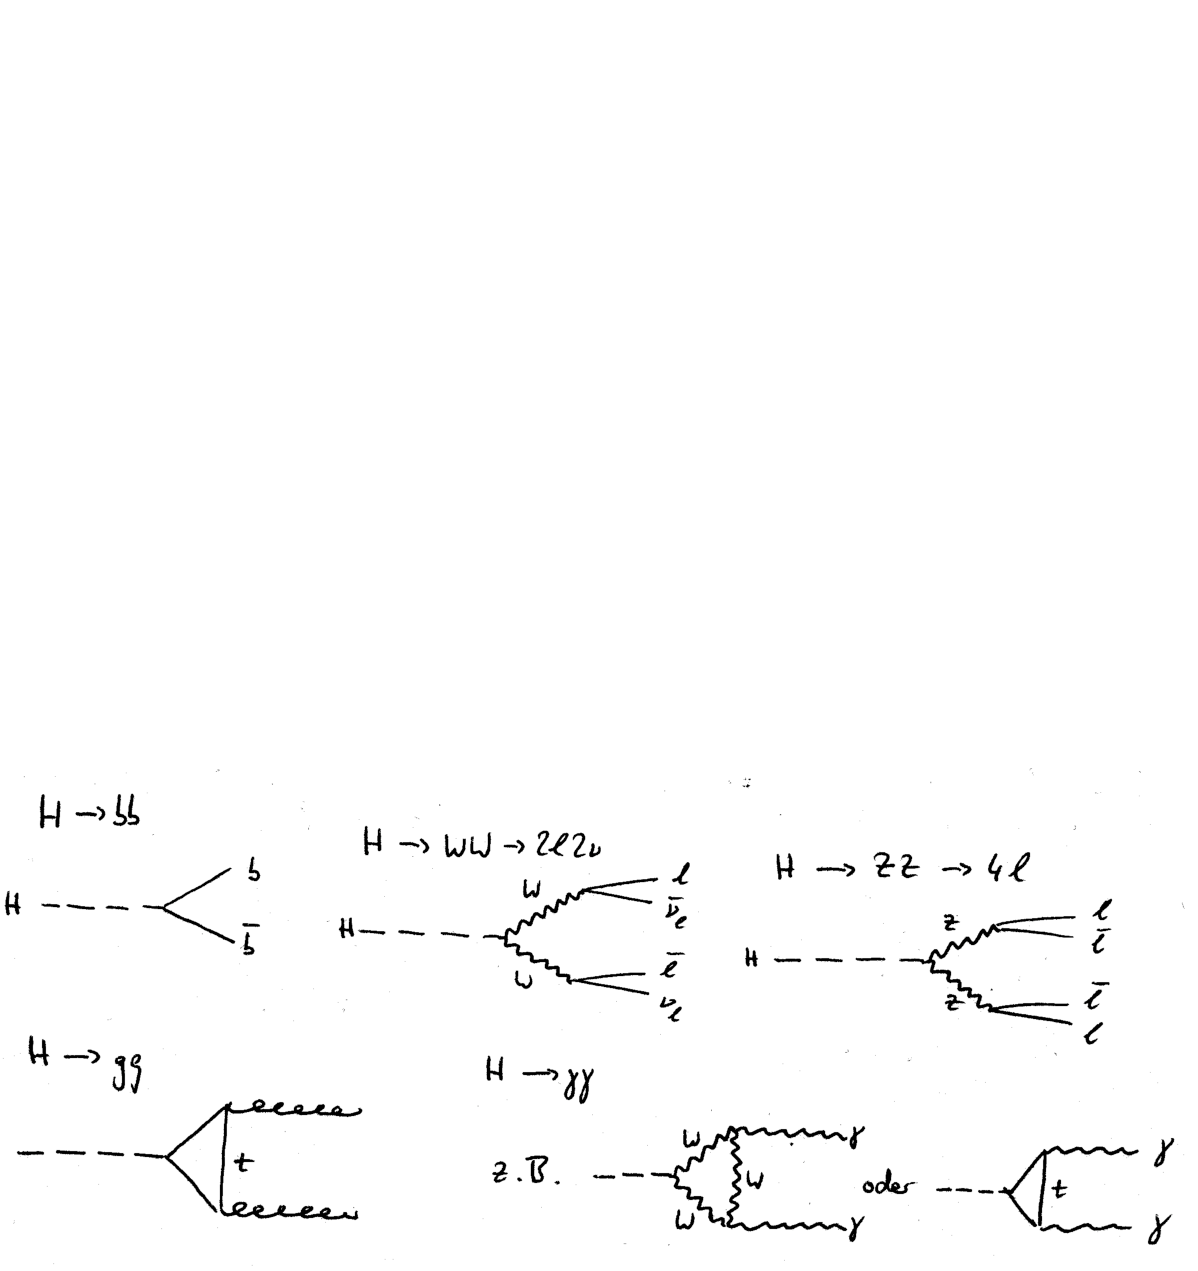
\includegraphics[height=6.5cm]{figures/LsgHiggs_decay.pdf}
		        \end{figure}
The most probable channel is bb because is the only one with one vertex and the interaction vertex of Higgs and fermion is directely proportional to the mass of the fermion therefore the bottom quork is the most probable. All the other particles are too massive for decay just with one vertex and we need loops

}

%\item 
%    Wie viele $pp \to b\bar{b}$ Ereignisse erwarten Sie bei einer integrierten Luminosität
%    von $\SI{50}{fb^{-1}}$? Wie viele Higgs-Ereignisse erwarten Sie in jedem der relevanten Higgs-Zerfallskanäle? 
%    \\(\textit{Hinweis: } Nehmen Sie an, dass der $b\bar{b}$-Wirkungsquerschnitt ungefähr $\SI{1e6}{\nano\barn}$ beträgt und der totale Wirkungsquerschnitt des Higgs bei $\SI{2e-2}{\nano\barn}$ liegt.)
      			
%    \solution{
%    How many $pp \to b\bar{b}$ events do you expect at a integrated luminosity of
	%$\SI{50}{fb^{-1}}$? How many Higgs events do you expect in each Higgs decay channel? (Assume a $b\bar{b}$ cross section of around \SI{1e6}{nb} and total cross section for the Higgs of \SI{2e-2}{nb}.)
   
    %            At an integrated luminosity of $\SI{50}{fb^{-1}}$ and a $bb$-XS
%		        of around \SI{1e6}{nb} you get around \num{5e13} $bb$ events. For a
		        %\SI{125}{GeV} Higgs the total XS is \SI{2e-2}{nb} which is leads to
		        %around \num{1000000} Higgs events.
		        %Around \SI{60}{\percent} (\num{600000} Events) decay through the
		        %$b\overline{b}$ channel, \SI{20}{\percent} through the $WW$ channel,
		        %\SI{7}{\percent} through the $gg$ or $\tau\tau$ channel, \SI{3}{\percent}
		        %through the $c\overline{c}$, or  $ZZ$ channel and \SI{0.2}{\percent}
		        %(\num{2000}) through the $\gamma\gamma$ channel.}
          
\item Die Oberfläche der Erde ist ständig einer großen Menge an energiereichen Teilchen ausgesetzt, die als kosmische Strahlung (CR) bezeichnet wird. Wenn diese CR mit den Molekülen der Atmosphäre in Wechselwirkung tritt, wird eine große Menge subatomarer Teilchen erzeugt, darunter auch das Higgs-Boson. Geht man davon aus, dass die Protonen in den Molekülen der Atmosphäre aufgrund der hohen Energie der CR, die mit diesen Hadronen kollidieren, freie Teilchen sind, können die Kollisionen als Proton-Proton-Kollisionen betrachtet werden. Der dominierende Teil des Wirkungsquerschnitts der Higgs-Produktion ist die Gluonenfusion, und das Verzweigungsverhältnis der Higgs-Bosonen-Produktion durch Gluonenfusion zum gesamten p-p-Wirkungsquerschnitt $\frac{\sigma_{Higgs}}{\sigma_{total}}$ ist in der folgenden Grafik dargestellt

\begin{figure}[htbp]
		            \centering
		            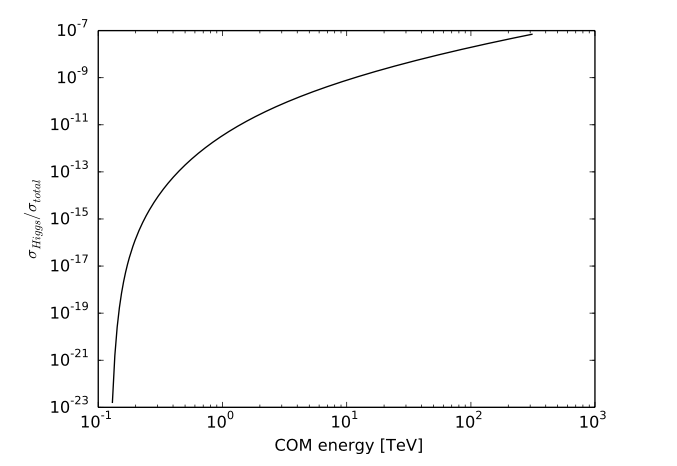
\includegraphics[height=6.5cm]{figures/Higgs_BR}
\end{figure}
Die Anzahl der pro Zeiteinheit $\mathrm{d}t$ erzeugten Higgs-Teilchen $N_H$ ist gleich

\begin{equation}
\frac{\mathrm{d}N_H}{\mathrm{d}t}=\frac{\sigma_{Higgs}}{\sigma_{total}}\frac{\mathrm{d}\phi}{\mathrm{d}t}\,,
\end{equation}
wobei $\frac{\mathrm{d}\phi}{\mathrm{d}t}$ der Fluss von CR pro Zeiteinheit ist und das $\frac{\sigma_{Higgs}}{\sigma_{total}}$ zuvor definiert wurde.
Der Fluss der CR pro Zeiteinheit, Oberfläche $A$, Energie des Massenschwerpunkts der Kollision $E_{COM}$ und Raumwinkel $\mathrm{d}\Omega$ ist gegeben durch
\begin{equation}
\frac{\mathrm{d}\phi^4}{\mathrm{d}t\mathrm{d}A\mathrm{d}E_{COM}\mathrm{d}\Omega}\sim 10^{-9}.
\end{equation}
Schätzen Sie die Anzahl der Higgs-Bosonen ab, die an einem Tag in 10 km Höhe produziert werden, wenn Sie nur CR aus Quellen innerhalb der Galaxie ($E_{CR}\sim \SI{3e10}{\electronvolt}$) berücksichtigen und annehmen, dass der Fluss aus allen Richtungen isotrop ist (keine Abhängigkeit des $\phi$ von der Fläche und dem Raumwinkel).
\textit{(Hinweise: Die Beziehung zwischen der Energie im Massenschwerpunkt und der Energie des CR ist $E_{COM}=\sqrt{(E_{CR} +m_P)2m_P}$. Der Radius der Erde beträgt \SI{6371}{\kilo\meter}. Die Masse des Protoms $m_P$ ist gleich \SI{0.938}{\giga\electronvolt/c^2}.)} (4P)
  \solution{
\begin{equation}
A =(6371 km + 10 km)^2\pi = 1.28 \times 10^{11} m^2
\end{equation}
\begin{equation}
      E_{COM}=\sqrt{(E_{CR} +m_P)2m_P} =2.3\times 10^4 GeV
\end{equation}
      From the graph, the value of $\frac{\sigma_{Higgs}}{\sigma_{total}}$ is approximately $10^{-8}$.
     \begin{align*}
\frac{\mathrm{d}N_H}{\mathrm{d}t}&=\frac{\sigma_{Higgs}}{\sigma_{total}}\times\frac{10^{-9}}{m^2 \times s \times sr \times GeV} \times A \times 4\pi \times E_{COM}\\
&= 10^{-8}\times \frac{10^{-9}}{m^2 \times s \times sr \times GeV} \times 1.28 \times 10^{11} m^2\times 4\pi \times 2.3\times10^4 GeV = 0.36 Higgs\cdot s^{-1}
\end{align*}
In a day there are 86400 seconds, so in one day approximatelly 31k Higgs are produced
  }
\end{enumerate}
\newpage
\null\newpage
\null\newpage
\section{Mandelstam-Variablen (10P)}
Die sogenannten Mandelstam-Variablen $s,\,t$ und $u$ werden in der Teilchenphysik bei der Beschreibung von Streuprozessen von zwei Körpern nach dem Schema $1 + 2 \rightarrow 3 + 4$ verwendet und sollen im Folgenden näher betrachtet werden.
%
\begin{align*}
 s &= \left(P_1 + P_2 \right)^2 \\
 t &= \left(P_1 - P_3 \right)^2 \\
 u &= \left(P_1 - P_4 \right)^2
\end{align*}
%
Hierbei werden die Viererimpulse der Teilchen mit $P_1$ bis $P_4$ beschrieben.
%
\begin{enumerate}[label=\alph*)]
 \item Leiten sie die Beziehung $s+t+u = \sum_{i=1}^4 m_i^2$ her, wobei $m_i$ die Massen der Teilchen 1-4 sind. (2P) \\(\textit{Hinweis: }Beachten Sie die Viererimpulserhaltung!)
 \solution{
 Viererimpulserhaltung: $P_1 + P_2 = P_3 + P_4$
 \begin{align*}
  s + t + u &=  \left(P_1 + P_2 \right)^2 +  \left(P_1 - P_3 \right)^2 +  \left(P_1 - P_4 \right)^2 \\
            &= m_1^2 + m_2^2 +2\,P_1\,P_2 +m_1^2 + m_3^2 -2\,P_1\,P_3+ m_1^2 + m_4^2 -2\,P_1\,P_4 \\
            &= 3\,m_1^2 + m_2^2 + m_3^2+m_4^2 + 2\,P_1\,\left(P_2 - P_3 - P_4 \right) \\
            &= 3\,m_1^2 + m_2^2 +m_3^2+m_4^2 - 2\,P_1\,P_1 \\
            &= m_1^2 + m_2^2+m_3^2+m_4^2 =\sum_{i=1}^4 m_i^2
 \end{align*}
 }
 \item Drücken Sie nun die Energie $E_1$ des Teilchens 1 im Schwerpunktssystem der eingehenden Teilchen durch $s$, sowie die Massen $m_1$ und $m_2$ aus. (3P)
 \solution{
 Im Schwerpunktssystem heben sich die Impulse der einlaufenden Teilchen auf, also  $\vec{p}_1 - \vec{p}_2 = \vec{0}$. Sie sind also betragsmäßig gleich und entgegengesetzt orientiert. Damit vereinfacht sich die Formel für die Mandelstam-Variable $s$ zu:
 \begin{align*}
     s &= (p_1 + p_2)^2\\
       &= (E_1 + E_2)^2\\
       &= E^2_1 + E^2_2 + 2E_1E_2
 \end{align*}
 Nutzen wir nun das $|\vec{p}_2| = |\vec{p}_1| = |\vec{p}|$ ist, können wir die Energie-Impuls-Beziehung des zweiten Teilchens umschreiben zu
 \begin{align*}
 E^2_2 &= m^2_2 + |\vec{p}_2|^2\\
       &= m^2_2 + |\vec{p}|^2\\
       &= m^2_2 + E^2_1 - m^2_1
 \end{align*}
 Einsetzen in unsere Rechnung:
 \begin{align*}
     s = 2E^2_1 + m^2_2 - m^2_1 + 2E_1\sqrt{E^2_1 + m^2_2 - m^2_1}
 \end{align*}
 und nach einigen Umformungen
 \begin{align*}
     E_1 = \frac{s + m^2_1 - m^2_2}{2\sqrt(s)}
 \end{align*}
 }
\end{enumerate}
%
Betrachten Sie im Folgenden die M\o ller-Streuung $e^- + e^- \rightarrow e^- + e^-$ und berücksichtigen Sie nur die elektromagnetische Wechselwirkung.
%
\begin{enumerate}[label=\alph*),resume]
 \item  Zeichnen Sie die möglichen Feynman-Diagramme erster Ordnung zu diesem Prozess. Mit welcher Mandelstam-Variable können diese jeweils in Verbindung gebracht werden? Was ist der Unterschied zur Elektron-Positron-Streuung? (2P)
 \solution{
 \begin{figure}[!h]
 \begin{tikzpicture}
  \begin{feynman}
   \vertex (a1) {\(e^-\)};
   \vertex[right=4cm of a1] (a3) {\(e^-\)};
   \vertex at ($(a1)!0.5!(a3) - (0, 1cm)$) (a2);
   \vertex[below=4cm of a1] (b1) {\(e^-\)};
      \vertex[right=4cm of b1] (b3) {\(e^-\)};
   \vertex at ($(b1)!0.5!(b3) + (0, 1cm)$) (b2);
   \diagram*{

   (a1) -- [fermion] (a2) -- [fermion] (a3);
   (b1) -- [fermion] (b2) -- [fermion] (b3);
   (a2) -- [boson, edge label=\(\gamma\)] (b2);
   };
  \end{feynman}
 \end{tikzpicture}
\hspace*{2cm}
 \begin{tikzpicture}
  \begin{feynman}
   \vertex (a1) {\(e^-\)};
   \vertex[right=4cm of a1] (a3) {\(e^-\)};
   \vertex at ($(a1)!0.5!(a3) - (0, 1cm)$) (a2);
   \vertex[below=4cm of a1] (b1) {\(e^-\)};
      \vertex[right=4cm of b1] (b3) {\(e^-\)};
   \vertex at ($(b1)!0.5!(b3) + (0, 1cm)$) (b2);
   \diagram*{

   (a1) -- [fermion] (a2) -- [fermion] (b3);
   (b1) -- [fermion] (b2) -- [fermion] (a3);
   (a2) -- [boson, edge label=\(\gamma\)] (b2);
   };
  \end{feynman}
 \end{tikzpicture}
\end{figure}
Das linke Feynman-Diagram kann mit der Mandelstam-Variable $t$, das rechte Feynman-Diagram mit der Mandelstam-Variable $u$ identifiziert werden. Ein $s$-Kanal liegt hier nicht vor. Bei der Bhabha-Streuung liegen keine identischen Teilchen im Endzustand vor, sodass kein $u$-Kanal möglich ist. Dafür gibt es aber ein Anihilations-Diagramm.
 }
 \item  Berechnen Sie im Folgenden die Größen $s$, $t$ und $u$ im Schwerpunktssystem der einlaufenden Elektronen als Funktion der Dreier-Impulse und des Streuwinkels $\theta$. Nehmen Sie hierfür eine elastische Streuung an. (2P)
\solution{
          Zunächst wird $s$ im Schwerpunktssystem berechnet.
          \begin{align*}
           s = \left(P_1 + P_2 \right)^2 = m_1^2 + m_2^2 + 2\,E_1\,E_2 - 2\,\vec{p}_1\,\vec{p}_2
          \end{align*}

          Da Elektronen sind identische Teilchen und besitzen die Masse $m_e$, also demnach auch dieselbe Energie $E_e$ im Schwerpunktssystem. Im Schwerpunktssystem sind die Impulse zudem entgegengesetzt gleich groß.

          \begin{align*}
           \sqrt{s} &= m_1^2 + m_2^2 + 2\,E_1\,E_2 - 2\,\vec{p}_1\,\vec{p}_2 \\
           \sqrt{s} &= 2\,m_e^2 + 2\,E_e^2 + 2|\,p_e|^2 \\
           \sqrt{s} &= 4\,(m_e^2 + |\vec{p}_e|^2)\\
           \sqrt{s} &= 4\,E_e^2
          \end{align*}

          Im letzten Schritt wurde wieder die Energie-Impuls-Beziehung ausgenutzt.\\
          Da es sich um einen elastischen Streuprozess handelt sind sowohl die Energien und Impulsbeträge des ein- und auslaufenden Elektrons identisch $E_i = E_e$ und $|vec{p}_i| = |vec{p}_e|$. Dies soll nun im $t$-Kanal betrachtet werden.

           \begin{align*}
            t &= \left(P_1 - P_3 \right)^2 = m_1^2 +m_2^2 - 2\,E_1\,E_3 + 2\,\vec{p}_1\,\vec{p}_2 \\
              &= 2\,m_e^2 - 2\,E_e^2 + 2\,|vec{p}_e|^2\,\cos\theta \\
              &= -2\,|vec{p}_e|^2 (1 - \cos\theta)
            \end{align*}
          Eine analoge Rechnung liefert
            \begin{align*}
             u = -2\,|vec{p}_e|^2 (1 + \cos\theta)
            \end{align*}
}
          
 \item  Wie hängt die Schwerpunktsenergie mit den Mandelstam-Variablen zusammen? (1P)
 \solution{
 $E_S = \sqrt{s}$
 }
\end{enumerate}

\newpage
\null\newpage
\null\newpage
\section{Radioaktive Zerfälle (10P)}

In einem ursprünglich kein Blei enthaltendem Uran-Mineral entstehen die Blei-Isotope \ce{^{207}Pb} und \ce{^{206}Pb} durch den radioaktiven Zerfall der folgenden Uran-Isotope:
\begin{itemize}
          \item \ce{^{235}U} \qquad Häufigkeit heute: $0,72\%$, Halbwertszeit: $7,038\cdot10^8$ \unit{a}
          \item \ce{^{238}U} \qquad Häufigkeit heute: $99,28\%$, Halbwertszeit: $4,0468\cdot10^9$ \unit{a} 
\end{itemize}
Das Mineral sei $600$ Mio. Jahre alt.

\begin{enumerate}
\item Stellen Sie die Zerfallsgesetze der Uran-Isotope auf. (2P)

\item \ce{^{235}U} zerfällt über die natürliche Uran-Actinium-Reihe zu \ce{^{207}Pb}, \ce{^{238}U} über die natürliche Uran-Radium-Reihe zu \ce{^{206}Pb}. Erklären Sie kurz, was natürliche Zerfallsreihen sind. Stellen Sie weitergehend die Zerfallsgesetze der Blei-Isotope auf. (2P)

\item Welches Masseverhältnis
Blei zu Uran enthält das Mineral heute? (2P)

\item Wie groß ist das
Häufigkeitsverhältnis \ce{^{207}Pb} zu \ce{^{206}Pb}? (2P)
  \solution{
      Test solution
  }

\item Bestimmen Sie nun das Alter der Erde unter den Annahmen, dass an
ihrem Anfang \ce{^{235}U} und \ce{^{238}U} gleich häufig vorkamen und zum heutigen Zeitpunkt die für Uran angegebenen Häufigkeiten gelten. (2P)
\end{enumerate}
\newpage
\null\newpage
\null\newpage
\cleardoubleplainpage

\newcommand {\1}{\protect\raisebox{-1.4ex}[1.0ex][0ex]{"}}
\newcommand{\kev}{~\textrm{keV}}
\newcommand{\mev}{~\textrm{MeV}}
\newcommand{\gev}{~\textrm{GeV}}
\newcommand{\ev} {~\textrm{eV}}
\newcommand{\half}{\frac{1}{2}}
%\newcommand{\s}{~\textrm{s}}



\begin{center}
\hspace*{3cm}{\small Einige Elementarteilchen und deren Eigenschaften} 
\end{center}
\scriptsize
$$
\begin{array}{|l|c|c||c|c|c|c|c|c|c|}\hline
 & &Quarks&  I^G(J^{PC}) & {\textrm{m}c}^2 &\tau (~\textrm{s})/\Gamma&{\textrm{(einige)}~ \mbox{\textrm{Zerfälle}}} \\ \hline
{(\textrm{Eich-})} & \gamma & & 0,1(1^{--}) & 0 & - & - \\
{\textrm{bosonen}} & g & & 0(1^{--}) & 0 & - & - \\
& W^\pm & & J=1 & 80.40\gev & 2.14\gev & \ell\nu, \textrm{Hadronen}: q_1\bar{q}_2, \cdots\\
 & Z ^0 & &  J=1 &91.188\gev & 2.495\gev & \ell^+\ell^-, \textrm{Hadronen}: q\bar{q}, \cdots  \\\hline
\textrm{Higgs}  &H^0& & J=0 &\approx 125\gev  &<0.013\gev&  \ell^+\ell^-, q\bar{q}, ZZ^*,WW^*, \gamma\gamma, \cdots \\\hline
\textrm{Leptonen}  &  \nu_e &&  (\half^+)  & <2\ev & -  & -\\
 (\ell)& e^- & &(\half^+) & 0.511\mev & - & - \\
& \nu_\mu & & (\half^+)  & <2\ev & - & -  \\
& \mu^- & & (\half^+) & 105.658\mev & 2.197\cdot10^{-6}~\textrm{s} & e^-\bar{\nu}_e\nu_\mu\\
& \nu_\tau & &  (\half^+) & <2\ev & - & - \\
& \tau^- & &(\half^+)&1776.84\mev & 290.6\cdot10^{-15}~\textrm{s} & \ell^-\bar{\nu}_\ell\nu_\tau, \rho^-\nu_\tau, \pi^-\nu_\tau,\cdots \\ \hline
\textrm{Mesonen}&  \pi^\pm & u\bar{d}\, \textrm{bzw}\,\bar{u}d & 1^-(0^-) & 139.6\mev  & 2.6\cdot10^{-8}~\textrm{s} & \\% \mu^\pm\nu_\mu \\
& \pi^0 & u\bar{u},d\bar{d} & 1^-(0^{-+}) & 134.977\mev & 8.4\cdot10^{-17}~\textrm{s} & \\% \gamma\gamma,\gamma e^+e^-\\ 
& \eta & u\bar{u},d\bar{d},s\bar{s} & 0^+(0^{-+}) & 547.9\mev & 1.30\kev & \gamma\gamma, 3\pi^0, \pi^+\pi^-\pi^0,\cdots \\
& \eta\prime & u\bar{u},d\bar{d},s\bar{s} & 0^+(0^{-+}) & 957.7\mev & 205\kev & \pi^+\pi^-\eta,\rho\gamma,\pi^0\pi^0\eta,\cdots  \\
& \rho^\pm & u\bar{d}\, \textrm{bzw}\,\bar{u}d & 1^+ (1^-) & 775.5\mev & 149.4\mev & \pi^\pm\pi^0 \\ 
& \rho^0& u\bar{u},d\bar{d}& 1^+(1^{--}) & 775.5\mev & 149.4\mev & \\% \pi^+\pi^-\\
& \omega &\approx u\bar{u},d\bar{d} & 0^-(1^{--}) &782.6\mev & 8.49\mev & \\%\pi^+\pi^-\pi^0, \pi^0\gamma,\pi^+\pi^- \\
& \phi &\approx s\bar{s} & 0^-(1^{--}) & 1019.46\mev & 4.26\mev & K^+K^-,  K^0_L K^0_S, \pi^+\pi^-\pi^0,\cdots \\[1.5ex]
& J/\psi & c\bar{c} & 0^-(1^{--})  & 3096.92\mev & 93.2\kev & \ell^+\ell^-, \textrm{Hadronen}, \cdots \\
& \psi(2S) & c\bar{c}&  0^-(1^{--})  & 3686.1\mev & 317\kev & J/\psi \pi\pi,\textrm{Hadronen}, \cdots  \\
& K^\pm & u\bar{s}\, \textrm{bzw}\,\bar{u}s & \half(0^-) & 493.7\mev & 1.238\cdot 10^{-8}~\textrm{s} & \mu^\pm\nu_\mu,\pi^\pm\pi^0,\cdots\\
& K^0/\bar{K}^0 & d\bar{s}\, \textrm{bzw}\, \bar{d}s &  \half(0^-) & 497.61\mev & &\\
&K^0_S & d\bar{s},\bar{d}s & \half(0^-) & 497.61\mev & 0.8958\cdot10^{-10}~\textrm{s} & \\ %\pi^+\pi^-,\pi^0\pi^0\\
&K^0_L &d\bar{s},\bar{d}s & \half(0^-) & 497.61\mev & 5.115\cdot10^{-8}~\textrm{s} & \\%\pi\pi\pi,\pi^-\ell^+\nu_\ell/ \pi^+\ell^-\bar{\nu}_\ell, (\pi\pi)\\
& K^{*\pm} & u\bar{s}\, \textrm{bzw}\,\bar{u}s & \half(1^-) & 891.7\mev & 50.8\mev & K\pi \\
& K^{*0}/ \bar{K}^{*0} &  d\bar{s} / \bar{d}s & \half(1^-) & 895.9\mev & 48.7\mev & K\pi \\[1.5ex]
& D^\pm&c\bar{d} \, \textrm{bzw} \,  \bar{c}d& \half(0^-) & 1869.6\mev & 1.04\cdot10^{-12}~\textrm{s} &  \bar{K}^{0}\ell^\pm\nu_\ell, K^\pm\pi^+\pi^+,\cdots \\
& D^0 / \bar{D^0}&c\bar{u}\, \textrm{bzw} \,  \bar{c}u  & \half(0^-) & 1864.8\mev & 0.41\cdot10^{-12}~\textrm{s} & K^\mp\ell^\pm\nu_\ell, K^\mp\pi^\pm,\cdots \\
& D^{*+}&c\bar{d}  & \half (1^-) & 2010.3\mev  & 96\kev &  D^0\pi^+, D^+\pi^0,D^+\gamma\\ 
& D^{*0} & c\bar{u}& \half (1^-) & 2007.0\mev & <2.1\mev & D^0\pi^0, D^0\gamma \\
&D_{s}^{\pm}& c\bar{s}\, \textrm{bzw}\,\bar{c}s  & 0 (0^-) & 1968.5\mev & 0.50\cdot10^{-12}~\textrm{s} &  \phi\pi^\pm, K^*K,\cdots \\[1.5ex]

& B^\pm& \bar{b}u \, \textrm{bzw} \, b\bar{u}& \half (0^-) & 5279.2\mev & 1.64\cdot 10^{-12}~\textrm{s} & \bar{D}^{*0}\ell^\pm\nu_\ell, \bar{D}^{*0}\rho^\pm,J/\psi X,\cdots \\
& B^\pm_c& c\bar{b}\,\textrm{bzw}\,\bar{c}b & 0(0^-) & 6274\mev & 0.5\cdot 10^{-12}~\textrm{s} & J\!/\!\psi\ell^+\nu_\ell \\
& B^0/\bar{B^0} &\bar{b}d\,\textrm{bzw}\,b\bar{d} &  \half (0^-) & 5279.5\mev & 1.52\cdot 10^{-12}~\textrm{s} & {D^{*}}\ell\nu_\ell,J/\psi K^0_S,\cdots \\
& B_{s}^{0}/\bar{B}_{s}^0 &\bar{b}s\,\textrm{bzw}\,b\bar{s} &  \half (0^-) & 5366.7\mev & 1.497\cdot 10^{-12}~\textrm{s} & {D_s}\ell\nu_\ell,D_s\pi,J/\psi\phi\cdots \\ \hline
\textrm{Baryonen }& p  &uud & \half (\half^+) & 938.27\mev & >10^{31}~\textrm{a} & -  \\
& n &udd  &  \half (\half^+) &  939.56\mev & 885.7~\textrm{s} & pe^-\bar{\nu}_e \\
& \Lambda &uds &  0  (\half^+) &  1115.68\mev & 2.63\cdot10^{-10}~\textrm{s} & p\pi^-,n\pi^0 \\
&\Sigma^+ &  uus&  1 (\half^+) &  1189.37\mev & 0.802\cdot10^{-10}\textrm{s} & p\pi^0, n\pi^+ \\
&\Sigma^0&  uds&  1 (\half^+) &  1192.64\mev & 7.4\cdot10^{-20}\textrm{s} & \Lambda\gamma\\
&\Sigma^- &  dds&  1 (\half^+) &  1197.45\mev & 1.48\cdot10^{-10}\textrm{s} & n\pi^-\\
&\Xi^0 & uss& \half (\half^+) &   1314.8\mev & 2.90\cdot10^{-10}\textrm{s} & \Lambda\pi^0\\
&\Xi^- & dss& \half (\half^+) &   1321.3\mev & 1.64\cdot10^{-10}\textrm{s} & \Lambda\pi^0\\
&\Omega^- & sss& 0  ({\frac{3}{2}}^+) &   1672.5\mev & 0.82\cdot10^{-10}\textrm{s} & \Lambda K^-, \Xi^0\pi^-,\Xi^-\pi^0 \\
&\Delta^{-} & ddd& \frac{3}{2}({\frac{3}{2}}^+) &1232\mev & 120\mev & n\pi^-  \\
&\Delta^{+} & uud & \frac{3}{2}{{\frac{3}{2}}^+} & 1232\mev & 120\mev & \\
&\Delta^{++} & uuu& \frac{3}{2}({\frac{3}{2}}^+) &1232\mev & 120\mev & p\pi^+  \\
& \Xi^{0}_c &csd & \half (\half^+)  & 2471.8\mev & 0.11\cdot10^{-12}\textrm{s} & \Lambda \bar{K}^0,  \Xi^-e^+\nu_e,\cdots \\
& \Lambda_b & udb& 0(\half^+) & 5624\mev & 1.2\cdot10^{-12}\textrm{s} & \Lambda J/\psi, pD^0\pi^-,\Lambda_c \ell^-\bar{\nu}_\ell,\cdots \\
& \Omega_b^-/\overline{\Omega_b^-} & ssb/\bar{s}\bar{s}\bar{b} & 0(\half^+) & 6046\mev & 1.64\cdot10^{-12}\textrm{s} & J\!/\!\psi\Omega^- \\
& \Sigma^+_b & uub & 1(\half^+) & 5810\mev & 1.3\cdot10^{-22}\textrm{s} & ? \\
& \Sigma^-_b & ddb & 1(\half^+) & 5815\mev & 1.2\cdot10^{-22}\textrm{s} & ? \\
& \Omega^0_c & ssc & 0(\half^+) & 2695\mev & 268\cdot10^{-15}\textrm{s} & \Omega^-e^+\nu_e \\
& \Xi_b^0 & usb& \half(\half^+) & 5788\mev & 1.5\cdot10^{-12}\textrm{s} & \Xi^- \ell^+\bar{\nu}_\ell,\cdots \\ \hline
\end{array}
$$



%\cleardoubleplainpage
%
\newcommand {\1}{\protect\raisebox{-1.4ex}[1.0ex][0ex]{"}}
\newcommand{\kev}{~\textrm{keV}}
\newcommand{\mev}{~\textrm{MeV}}
\newcommand{\gev}{~\textrm{GeV}}
\newcommand{\ev} {~\textrm{eV}}
\newcommand{\half}{\frac{1}{2}}
%\newcommand{\s}{~\textrm{s}}



\begin{center}
\hspace*{3cm}{\small Einige Elementarteilchen und deren Eigenschaften} 
\end{center}
\scriptsize
$$
\begin{array}{|l|c|c||c|c|c|c|c|c|c|}\hline
 & &Quarks&  I^G(J^{PC}) & {\textrm{m}c}^2 &\tau (~\textrm{s})/\Gamma&{\textrm{(einige)}~ \mbox{\textrm{Zerfälle}}} \\ \hline
{(\textrm{Eich-})} & \gamma & & 0,1(1^{--}) & 0 & - & - \\
{\textrm{bosonen}} & g & & 0(1^{--}) & 0 & - & - \\
& W^\pm & & J=1 & 80.40\gev & 2.14\gev & \ell\nu, \textrm{Hadronen}: q_1\bar{q}_2, \cdots\\
 & Z ^0 & &  J=1 &91.188\gev & 2.495\gev & \ell^+\ell^-, \textrm{Hadronen}: q\bar{q}, \cdots  \\\hline
\textrm{Higgs}  &H^0& & J=0 &\approx 125\gev  &<0.013\gev&  \ell^+\ell^-, q\bar{q}, ZZ^*,WW^*, \gamma\gamma, \cdots \\\hline
\textrm{Leptonen}  &  \nu_e &&  (\half^+)  & <2\ev & -  & -\\
 (\ell)& e^- & &(\half^+) & 0.511\mev & - & - \\
& \nu_\mu & & (\half^+)  & <2\ev & - & -  \\
& \mu^- & & (\half^+) & 105.658\mev & 2.197\cdot10^{-6}~\textrm{s} & e^-\bar{\nu}_e\nu_\mu\\
& \nu_\tau & &  (\half^+) & <2\ev & - & - \\
& \tau^- & &(\half^+)&1776.84\mev & 290.6\cdot10^{-15}~\textrm{s} & \ell^-\bar{\nu}_\ell\nu_\tau, \rho^-\nu_\tau, \pi^-\nu_\tau,\cdots \\ \hline
\textrm{Mesonen}&  \pi^\pm & u\bar{d}\, \textrm{bzw}\,\bar{u}d & 1^-(0^-) & 139.6\mev  & 2.6\cdot10^{-8}~\textrm{s} & \\% \mu^\pm\nu_\mu \\
& \pi^0 & u\bar{u},d\bar{d} & 1^-(0^{-+}) & 134.977\mev & 8.4\cdot10^{-17}~\textrm{s} & \\% \gamma\gamma,\gamma e^+e^-\\ 
& \eta & u\bar{u},d\bar{d},s\bar{s} & 0^+(0^{-+}) & 547.9\mev & 1.30\kev & \gamma\gamma, 3\pi^0, \pi^+\pi^-\pi^0,\cdots \\
& \eta\prime & u\bar{u},d\bar{d},s\bar{s} & 0^+(0^{-+}) & 957.7\mev & 205\kev & \pi^+\pi^-\eta,\rho\gamma,\pi^0\pi^0\eta,\cdots  \\
& \rho^\pm & u\bar{d}\, \textrm{bzw}\,\bar{u}d & 1^+ (1^-) & 775.5\mev & 149.4\mev & \pi^\pm\pi^0 \\ 
& \rho^0& u\bar{u},d\bar{d}& 1^+(1^{--}) & 775.5\mev & 149.4\mev & \\% \pi^+\pi^-\\
& \omega &\approx u\bar{u},d\bar{d} & 0^-(1^{--}) &782.6\mev & 8.49\mev & \\%\pi^+\pi^-\pi^0, \pi^0\gamma,\pi^+\pi^- \\
& \phi &\approx s\bar{s} & 0^-(1^{--}) & 1019.46\mev & 4.26\mev & K^+K^-,  K^0_L K^0_S, \pi^+\pi^-\pi^0,\cdots \\[1.5ex]
& J/\psi & c\bar{c} & 0^-(1^{--})  & 3096.92\mev & 93.2\kev & \ell^+\ell^-, \textrm{Hadronen}, \cdots \\
& \psi(2S) & c\bar{c}&  0^-(1^{--})  & 3686.1\mev & 317\kev & J/\psi \pi\pi,\textrm{Hadronen}, \cdots  \\
& K^\pm & u\bar{s}\, \textrm{bzw}\,\bar{u}s & \half(0^-) & 493.7\mev & 1.238\cdot 10^{-8}~\textrm{s} & \mu^\pm\nu_\mu,\pi^\pm\pi^0,\cdots\\
& K^0/\bar{K}^0 & d\bar{s}\, \textrm{bzw}\, \bar{d}s &  \half(0^-) & 497.61\mev & &\\
&K^0_S & d\bar{s},\bar{d}s & \half(0^-) & 497.61\mev & 0.8958\cdot10^{-10}~\textrm{s} & \\ %\pi^+\pi^-,\pi^0\pi^0\\
&K^0_L &d\bar{s},\bar{d}s & \half(0^-) & 497.61\mev & 5.115\cdot10^{-8}~\textrm{s} & \\%\pi\pi\pi,\pi^-\ell^+\nu_\ell/ \pi^+\ell^-\bar{\nu}_\ell, (\pi\pi)\\
& K^{*\pm} & u\bar{s}\, \textrm{bzw}\,\bar{u}s & \half(1^-) & 891.7\mev & 50.8\mev & K\pi \\
& K^{*0}/ \bar{K}^{*0} &  d\bar{s} / \bar{d}s & \half(1^-) & 895.9\mev & 48.7\mev & K\pi \\[1.5ex]
& D^\pm&c\bar{d} \, \textrm{bzw} \,  \bar{c}d& \half(0^-) & 1869.6\mev & 1.04\cdot10^{-12}~\textrm{s} &  \bar{K}^{0}\ell^\pm\nu_\ell, K^\pm\pi^+\pi^+,\cdots \\
& D^0 / \bar{D^0}&c\bar{u}\, \textrm{bzw} \,  \bar{c}u  & \half(0^-) & 1864.8\mev & 0.41\cdot10^{-12}~\textrm{s} & K^\mp\ell^\pm\nu_\ell, K^\mp\pi^\pm,\cdots \\
& D^{*+}&c\bar{d}  & \half (1^-) & 2010.3\mev  & 96\kev &  D^0\pi^+, D^+\pi^0,D^+\gamma\\ 
& D^{*0} & c\bar{u}& \half (1^-) & 2007.0\mev & <2.1\mev & D^0\pi^0, D^0\gamma \\
&D_{s}^{\pm}& c\bar{s}\, \textrm{bzw}\,\bar{c}s  & 0 (0^-) & 1968.5\mev & 0.50\cdot10^{-12}~\textrm{s} &  \phi\pi^\pm, K^*K,\cdots \\[1.5ex]

& B^\pm& \bar{b}u \, \textrm{bzw} \, b\bar{u}& \half (0^-) & 5279.2\mev & 1.64\cdot 10^{-12}~\textrm{s} & \bar{D}^{*0}\ell^\pm\nu_\ell, \bar{D}^{*0}\rho^\pm,J/\psi X,\cdots \\
& B^\pm_c& c\bar{b}\,\textrm{bzw}\,\bar{c}b & 0(0^-) & 6274\mev & 0.5\cdot 10^{-12}~\textrm{s} & J\!/\!\psi\ell^+\nu_\ell \\
& B^0/\bar{B^0} &\bar{b}d\,\textrm{bzw}\,b\bar{d} &  \half (0^-) & 5279.5\mev & 1.52\cdot 10^{-12}~\textrm{s} & {D^{*}}\ell\nu_\ell,J/\psi K^0_S,\cdots \\
& B_{s}^{0}/\bar{B}_{s}^0 &\bar{b}s\,\textrm{bzw}\,b\bar{s} &  \half (0^-) & 5366.7\mev & 1.497\cdot 10^{-12}~\textrm{s} & {D_s}\ell\nu_\ell,D_s\pi,J/\psi\phi\cdots \\ \hline
\textrm{Baryonen }& p  &uud & \half (\half^+) & 938.27\mev & >10^{31}~\textrm{a} & -  \\
& n &udd  &  \half (\half^+) &  939.56\mev & 885.7~\textrm{s} & pe^-\bar{\nu}_e \\
& \Lambda &uds &  0  (\half^+) &  1115.68\mev & 2.63\cdot10^{-10}~\textrm{s} & p\pi^-,n\pi^0 \\
&\Sigma^+ &  uus&  1 (\half^+) &  1189.37\mev & 0.802\cdot10^{-10}\textrm{s} & p\pi^0, n\pi^+ \\
&\Sigma^0&  uds&  1 (\half^+) &  1192.64\mev & 7.4\cdot10^{-20}\textrm{s} & \Lambda\gamma\\
&\Sigma^- &  dds&  1 (\half^+) &  1197.45\mev & 1.48\cdot10^{-10}\textrm{s} & n\pi^-\\
&\Xi^0 & uss& \half (\half^+) &   1314.8\mev & 2.90\cdot10^{-10}\textrm{s} & \Lambda\pi^0\\
&\Xi^- & dss& \half (\half^+) &   1321.3\mev & 1.64\cdot10^{-10}\textrm{s} & \Lambda\pi^0\\
&\Omega^- & sss& 0  ({\frac{3}{2}}^+) &   1672.5\mev & 0.82\cdot10^{-10}\textrm{s} & \Lambda K^-, \Xi^0\pi^-,\Xi^-\pi^0 \\
&\Delta^{-} & ddd& \frac{3}{2}({\frac{3}{2}}^+) &1232\mev & 120\mev & n\pi^-  \\
&\Delta^{+} & uud & \frac{3}{2}{{\frac{3}{2}}^+} & 1232\mev & 120\mev & \\
&\Delta^{++} & uuu& \frac{3}{2}({\frac{3}{2}}^+) &1232\mev & 120\mev & p\pi^+  \\
& \Xi^{0}_c &csd & \half (\half^+)  & 2471.8\mev & 0.11\cdot10^{-12}\textrm{s} & \Lambda \bar{K}^0,  \Xi^-e^+\nu_e,\cdots \\
& \Lambda_b & udb& 0(\half^+) & 5624\mev & 1.2\cdot10^{-12}\textrm{s} & \Lambda J/\psi, pD^0\pi^-,\Lambda_c \ell^-\bar{\nu}_\ell,\cdots \\
& \Omega_b^-/\overline{\Omega_b^-} & ssb/\bar{s}\bar{s}\bar{b} & 0(\half^+) & 6046\mev & 1.64\cdot10^{-12}\textrm{s} & J\!/\!\psi\Omega^- \\
& \Sigma^+_b & uub & 1(\half^+) & 5810\mev & 1.3\cdot10^{-22}\textrm{s} & ? \\
& \Sigma^-_b & ddb & 1(\half^+) & 5815\mev & 1.2\cdot10^{-22}\textrm{s} & ? \\
& \Omega^0_c & ssc & 0(\half^+) & 2695\mev & 268\cdot10^{-15}\textrm{s} & \Omega^-e^+\nu_e \\
& \Xi_b^0 & usb& \half(\half^+) & 5788\mev & 1.5\cdot10^{-12}\textrm{s} & \Xi^- \ell^+\bar{\nu}_\ell,\cdots \\ \hline
\end{array}
$$

%\clearpage
\thispagestyle{empty}
\section*{Formeln, Konstanten}
Neben den hier aufgef\"uhrten Gr\"o{\ss}en finden Sie am Ende der Klausur eine Clebsch-Gordan-Tabelle und eine Liste von Teilchen und ihren Eigenschaften.

\begin{align*}
 c &= \SI{3e8}{m/s} \\
 \hbar &= \SI{1.055e-34}{Js} \\ &= \SI{6.582e-22}{MeV s}\\
 e &= \SI{1.6022e-19}{C} \\ 
 \frac{G_F}{(\hbar c)^3} &= \SI{1.166e-5}{GeV^{-2}} \\
 \alpha &= 1/137 \\
 N_A &= \SI{6.022e23}{mol^{-1}} \\
 \theta_C &= 0.22 \, {\text{ rad}} \\
 \epsilon_0 &= \SI{8.8541e-22}{\farad \metre^{-1}} \\ &= \SI{55.263}{e^2 eV^{-1} \micro m^{-1}} \\
\end{align*}
Die Einträge der CKM-Matrix lauten:
\begin{align*}
    V_\text{CKM} &= 
      \begin{pmatrix}
      V_{ud} & V_{us} & V_{ub} \\
      V_{cd} & V_{cs} & V_{cb} \\
      V_{td} & V_{ts} & V_{tb}
  \end{pmatrix}
\end{align*}
mit
\begin{align*}
 (|V_{ij}|) \approx
  \begin{pmatrix}
      1         & 0,2   & 0,008 \\
      0,2     & 1       & 0,04 \\
      0,008 & 0,04 & 1
  \end{pmatrix}
\end{align*}
Die Bethe-Weizs\"acker-Formel lautet:
\begin{align*}
E_\text{Bindung}\approx15,67\,\text{MeV}\cdot A - 17,23\,\text{MeV}\cdot A^{\frac 2 3} - 0,71\,\text{MeV}\cdot Z\cdot(Z-1) \cdot A^{-\frac 1 3} -  93,15\,\text{MeV}\cdot \frac{(N-Z)^2}{4A} + E_\text{Paar}
\end{align*}
mit
\begin{align*}
E_\text{Paar} = 
   \begin{cases}
     +11,2\,\text{MeV}\cdot A^{-\frac 1 2} & \text{f\"ur gg-Kerne}\\
     0  & \text{f\"ur ug- und gu-Kerne}\\
     -11,2\,\text{MeV} \cdot A^{-\frac 1 2} & \text{f\"ur uu-Kerne} 
   \end{cases}
\end{align*}

Einige Land\'e-Faktoren:\\
\centerline{\begin{tabular}{lc}\hline
Teilchen & $g$ \\ \hline
Elektron & -2.0023 \\
Myon     & -2.0023 \\
Neutron  & -3.8261 \\
Proton   & +5.5857 \\ \hline
\end{tabular}}

Abgestrahlte Leistung eines Teilchens: 
\begin{equation}
    P = \frac{e^2c}{6\pi\epsilon_0(m_0c^2)^4}\frac{E^4}{R^2}
\end{equation}
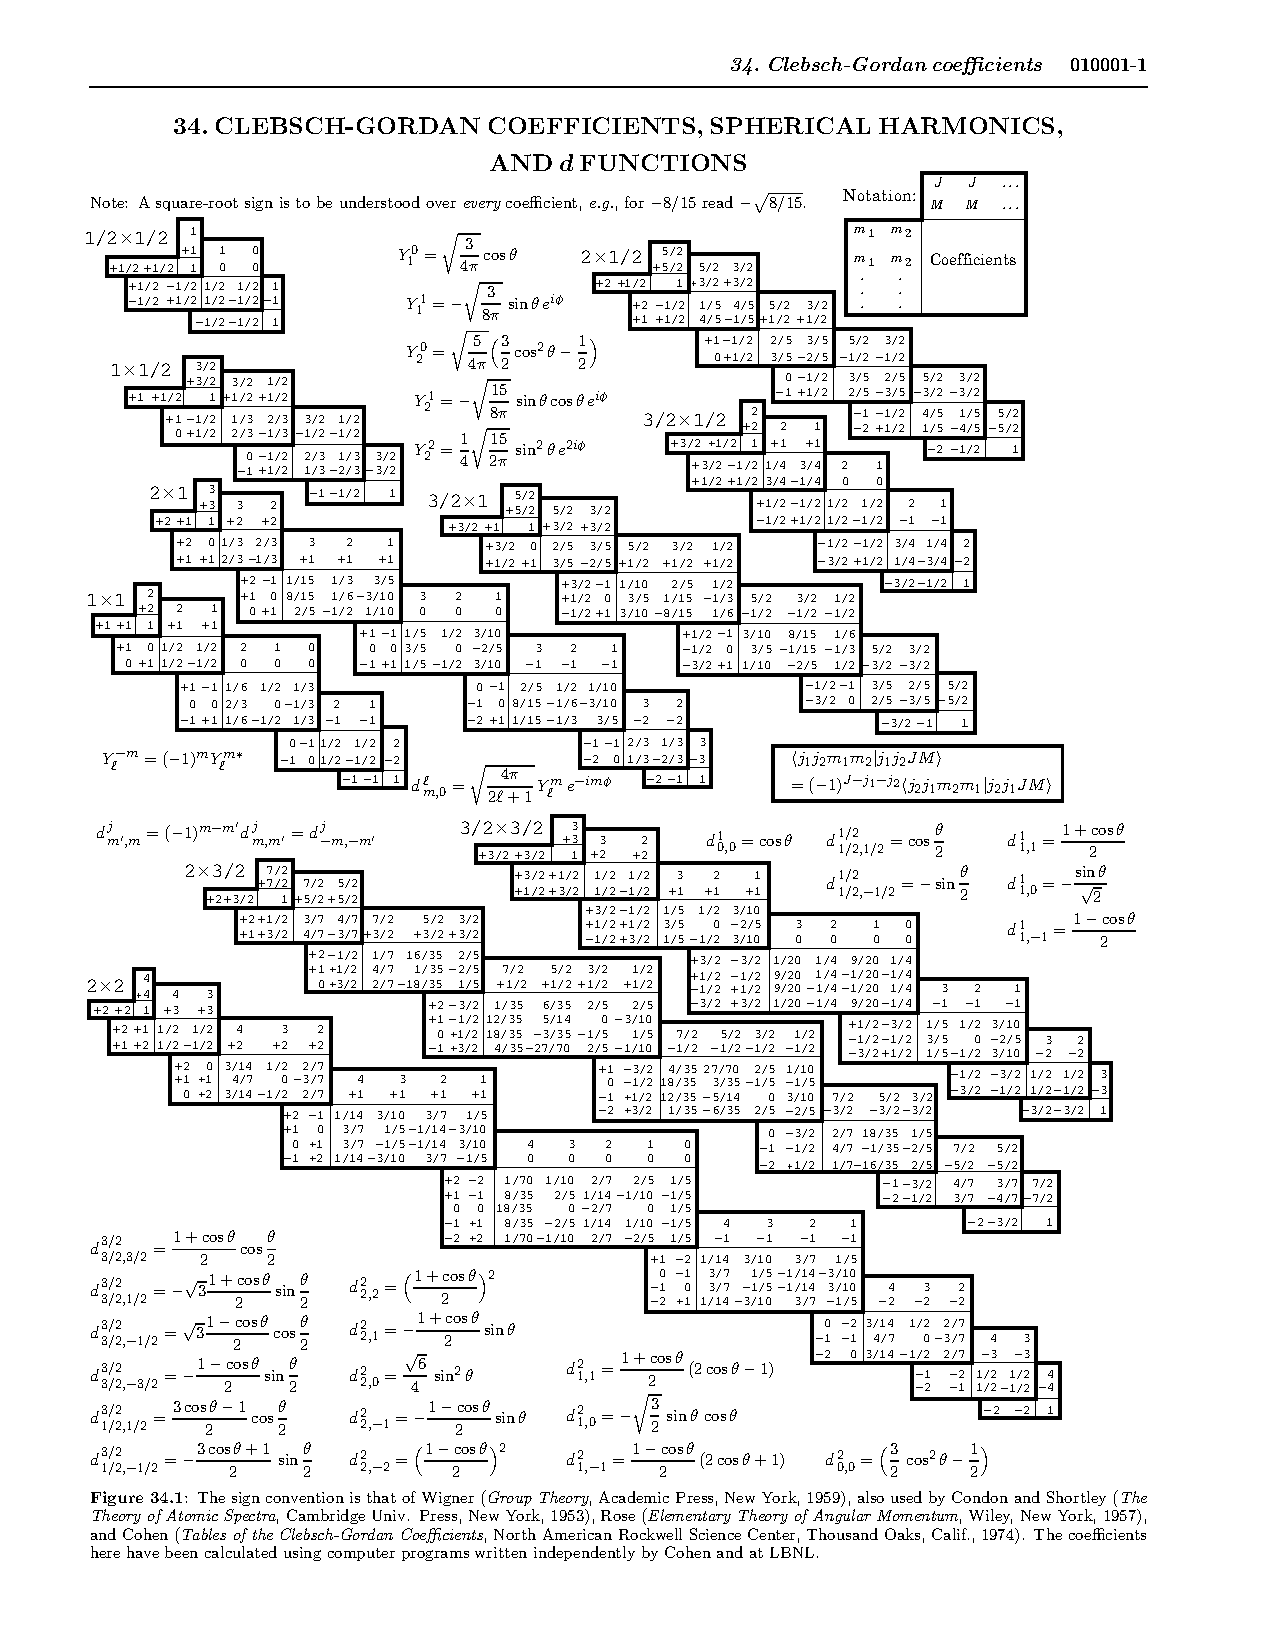
\includepdf[offset=0.0cm 0, scale=0.98]{clebsch.pdf}

\end{document}
